\question {
    某系统存在$4$个进程和$5$份可分配资源,当前的资源分配情况和最大需求如下表所示。求满足安全状态下$X$的最小值。请写出解题分析过程。
}

\begin{figure}[H]
    \centering
    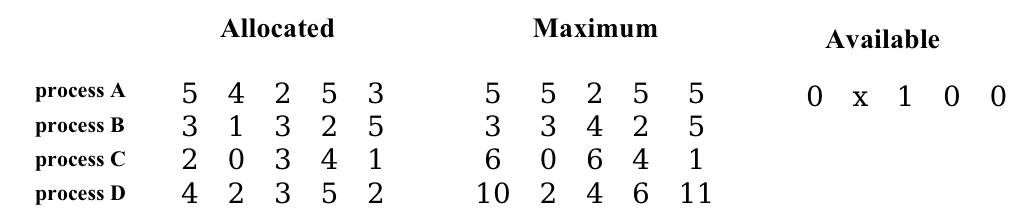
\includegraphics[width=0.8\textwidth]{img/6_1.png}
\end{figure}

\begin{solution}

根据题目,补充当前资源请求矩阵:

\begin{table}[H]
    \begin{center}
    \begin{tabular}{|c|c|c|c|c|c|c|c|c|c|c|c|c|c|c|c|c|c|c|c|c|c|c|c|}
    \hline
     & \multicolumn{ 5}{c|}{Allocated} &  & \multicolumn{ 5}{c|}{Maximum} &  & \multicolumn{ 5}{c|}{Request} &  & \multicolumn{ 5}{c|}{Available} \\ \hline
    A & 5 & 4 & 2 & 5 & 3 &  & 5 & 5 & 2 & 5 & 5 &  & 0 & 1 & 0 & 0 & 2 &  & 0 & x & 1 & 0 & 0 \\ \hline
    B & 3 & 1 & 3 & 2 & 5 &  & 3 & 3 & 4 & 2 & 5 &  & 0 & 2 & 1 & 0 & 0 &  &  &  &  &  &  \\ \hline
    C & 2 & 0 & 3 & 4 & 1 &  & 6 & 0 & 6 & 4 & 1 &  & 4 & 0 & 3 & 0 & 0 &  &  &  &  &  &  \\ \hline
    D & 4 & 2 & 3 & 5 & 2 &  & 10 & 2 & 4 & 6 & 11 &  & 6 & 0 & 1 & 1 & 9 &  &  &  &  &  &  \\ \hline
    \end{tabular}
    \end{center}
\end{table}


在所有资源请求矩阵中,只有分配给$B$是有可能安全的,此时要求$x>=2$。分配完如下所示:

\begin{table}[H]
    \begin{center}
    \begin{tabular}{|c|c|c|c|c|c|c|c|c|c|c|c|c|c|c|c|c|c|c|c|c|c|c|c|}
    \hline
     & \multicolumn{ 5}{c|}{Allocated} &  & \multicolumn{ 5}{c|}{Maximum} &  & \multicolumn{ 5}{c|}{Request} &  & \multicolumn{ 5}{c|}{Available} \\ \hline
    A & 5 & 4 & 2 & 5 & 3 &  & 5 & 5 & 2 & 5 & 5 &  & 0 & 1 & 0 & 0 & 2 &  & 3 & x+3 & 4 & 2 & 5 \\ \hline
    B & 0 & 0 & 0 & 0 & 0 &  & 0 & 0 & 0 & 0 & 0 &  & 0 & 0 & 0 & 0 & 0 &  &  &  &  &  &  \\ \hline
    C & 2 & 0 & 3 & 4 & 1 &  & 6 & 0 & 6 & 4 & 1 &  & 4 & 0 & 3 & 0 & 0 &  &  &  &  &  &  \\ \hline
    D & 4 & 2 & 3 & 5 & 2 &  & 10 & 2 & 4 & 6 & 11 &  & 6 & 0 & 1 & 1 & 9 &  &  &  &  &  &  \\ \hline
    \end{tabular}
    \end{center}
\end{table}

在所有资源请求矩阵中,只有分配给$A$是有可能安全的,此时$x+3>=1$一定成立。分配完如下所示:

\begin{table}[H]
    \begin{center}
    \begin{tabular}{|c|c|c|c|c|c|c|c|c|c|c|c|c|c|c|c|c|c|c|c|c|c|c|c|}
    \hline
     & \multicolumn{ 5}{c|}{Allocated} &  & \multicolumn{ 5}{c|}{Maximum} &  & \multicolumn{ 5}{c|}{Request} &  & \multicolumn{ 5}{c|}{Available} \\ \hline
    A & 0 & 0 & 0 & 0 & 0 &  & 0 & 0 & 0 & 0 & 0 &  & 0 & 0 & 0 & 0 & 0 &  & 8 & x+7 & 6 & 7 & 8 \\ \hline
    B & 0 & 0 & 0 & 0 & 0 &  & 0 & 0 & 0 & 0 & 0 &  & 0 & 0 & 0 & 0 & 0 &  &  &  &  &  &  \\ \hline
    C & 2 & 0 & 3 & 4 & 1 &  & 6 & 0 & 6 & 4 & 1 &  & 4 & 0 & 3 & 0 & 0 &  &  &  &  &  &  \\ \hline
    D & 4 & 2 & 3 & 5 & 2 &  & 10 & 2 & 4 & 6 & 11 &  & 6 & 0 & 1 & 1 & 9 &  &  &  &  &  &  \\ \hline
    \end{tabular}
    \end{center}
\end{table}

在所有资源请求矩阵中,只有分配给$C$是有可能安全的,此时$x+7>=4$一定成立。分配完如下所示:

\begin{table}[H]
    \begin{center}
    \begin{tabular}{|c|c|c|c|c|c|c|c|c|c|c|c|c|c|c|c|c|c|c|c|c|c|c|c|}
    \hline
     & \multicolumn{ 5}{c|}{Allocated} &  & \multicolumn{ 5}{c|}{Maximum} &  & \multicolumn{ 5}{c|}{Request} &  & \multicolumn{ 5}{c|}{Available} \\ \hline
    A & 0 & 0 & 0 & 0 & 0 &  & 0 & 0 & 0 & 0 & 0 &  & 0 & 0 & 0 & 0 & 0 &  & 10 & x+7 & 9 & 11 & 9 \\ \hline
    B & 0 & 0 & 0 & 0 & 0 &  & 0 & 0 & 0 & 0 & 0 &  & 0 & 0 & 0 & 0 & 0 &  &  &  &  &  &  \\ \hline
    C & 0 & 0 & 0 & 0 & 0 &  & 0 & 0 & 0 & 0 & 0 &  & 0 & 0 & 0 & 0 & 0 &  &  &  &  &  &  \\ \hline
    D & 4 & 2 & 3 & 5 & 2 &  & 10 & 2 & 4 & 6 & 11 &  & 6 & 0 & 1 & 1 & 9 &  &  &  &  &  &  \\ \hline
    \end{tabular}
    \end{center}
\end{table}

最后只剩下$D$未分配资源,分配给$D$是一定安全的,此时$x+7>=0$一定成立。

因此满足安全状态的最小值是$x=2$。

\end{solution}